
Uloshyppy ja ensimmäiset 1-2 sekuntia vapaapudotusta ovat ensimmäisillä hypyillä tyypillisesti sellaisia, että hyppääjä ei muista niistä mitään. Kokemuksen karttuessa ajantaju alkaa säilymään koko hyppysuorituksen ajan. Erityisesti hyppyuran alkuvaiheessa hyvä uloshyppy on yhtä kuin hyvä hyppy. Myöhemmin uloshypyn onnistuminen korostuu sekä muodostelmahypyillä että matalilla hypyillä (lyhyet vapaat). Uloshyppytyylistä riippumatta perusperiaate on hyödyntää suhteellista ilmavirtaa halutun asennon ja suunnan saamiseksi ja säilyttämiseksi. 


Uloshyppy on aina arvioitava suoritus ja sen tärkeimmät tekijät ovat ilmavirran suunnan huomioiminen sekä ponnistuksen suunta. Uloshyppyyn on varattava myös aina riittävästi aikaa, mikä on huomioitava uloshyppypaikkaa määriteltäessä. Tavoitteena on hallita kaikki uloshyppytyylit rutiinitasolla ja muistaa koko hyppysuoritus heti uloshypystä maahantuloon asti. 

\section{ Roikkumauloshyppy }
\label{uloshyppytyylit-roikkumauloshyppy}

\subsection{ Streevakone }
\label{uloshyppytyylit-streevakone}

\begin{enumerate}[label=\bfseries \arabic*)]
\item  Kiivetään streevakoneen ulkopuolelle (varoen repun osumista koneeseen) streevaa ja astinlautaa hyväksikäyttäen, rinta koneen etenemissuuntaan. 
\item  Lasketaan jalat yksitellen ilmavirtaan, ei hypätä. 
\item  Roikutaan käsillä noin hartialevyisellä otteella streevasta kiinni pitäen ja otetaan X-asento ja taivutus ilmavirran suuntaisesti. 
\item  Irrotetaan käsien ote yhtäaikaisesti. 
\item  Sitä mukaan kun asento kääntyy vaakatasoon (tyypillisesti noin 5 sekunnin jälkeen) otetaan perusasento. 
\end{enumerate}
\subsection{ Ongelmat }
\label{uloshyppytyylit-ongelmat}

\begin{itemize}
\item  Koukussa olevat jalat aiheuttavat takavoltin. 
\item  Negatiivinen taivutus kaataa asennon selälleen. 
\item  Astinlaudalta ilmavirtaan hyppääminen voi aiheuttaa ennenaikaisen tippumisen. 
\item  Käsillä ponnistaminen kaataa asennon selälleen. 
\end{itemize}
\section{ Suora uloshyppy }
\label{uloshyppytyylit-suora-uloshyppy}


\begin{Figure}\centering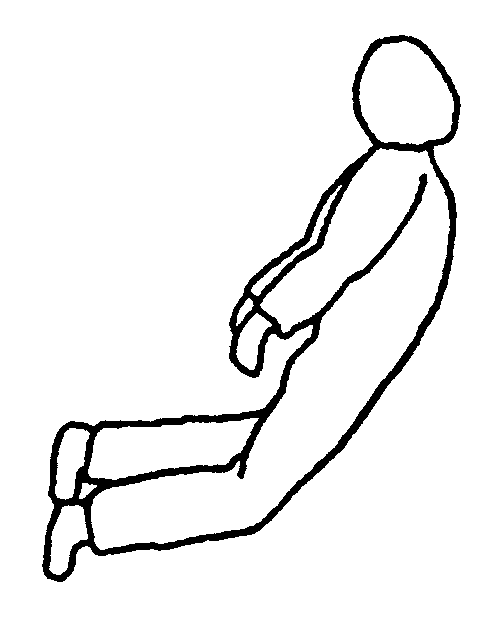
\includegraphics[width=0.7\textwidth]{UH-suora.png}\captionof{figure}{Suora uloshyppy}\end{Figure} 

\subsection{ Streevakone }
\label{uloshyppytyylit-streevakone}

\begin{enumerate}[label=\bfseries \arabic*)]
\item  Vasen jalka astimelle (pyörälle). 
\item  Kädet oviaukon reunalle. 
\item  Kohottaudutaan koneen (varoen repun osumista koneeseen) ulkopuolelle. 
\item  Käännetään rinta koneen etenemissuuntaan. 
\item  Ponnistetaan ilmavirran suuntaan taaksepäin. 
\item  Taivutus, pää taakse, jalat lähes suorina ja kädet taakse delta-asentoon. 
\item  Sitä mukaan kun asento kääntyy vaakatasoon (tyypillisesti noin 5 sekunnin jälkeen) otetaan perusasento. 
\end{enumerate}
\subsection{ Muut koneet }
\label{uloshyppytyylit-muut-koneet}

\begin{enumerate}[label=\bfseries \arabic*)]
\item  Siirrytään oviaukolle (varoen repun osumista koneeseen) kyykkyyn tai seisaalleen. 
\item  Ponnistetaan ilmavirran suuntaan eteenpäin, rinta koneen etenemissuuntaan. 
\item  Taivutus, pää taakse, jalat lähes suorina ja kädet taakse delta-asentoon. 
\item  Sitä mukaan kun asento kääntyy vaakatasoon (tyypillisesti noin 5 sekunnin jälkeen) otetaan perusasento. 
\end{enumerate}
\subsection{ Ongelmat }
\label{uloshyppytyylit-ongelmat}

\begin{enumerate}[label=\bfseries \arabic*)]
\item  Eteen jätetyt kädet aiheuttavat voltin. 
\item  Ponnistus sivulle aiheuttaa kaatumisen kyljelle. 
\item  Löysä uloshyppyasento aiheuttaa kaatumisen selälleen. 
\item  Streeva-koneessa heikko ponnistus voi johtaa osumiseen pyörätelineeseen. 
\end{enumerate}
\section{ Sukellusuloshyppy }
\label{uloshyppytyylit-sukellusuloshyppy}


\begin{Figure}\centering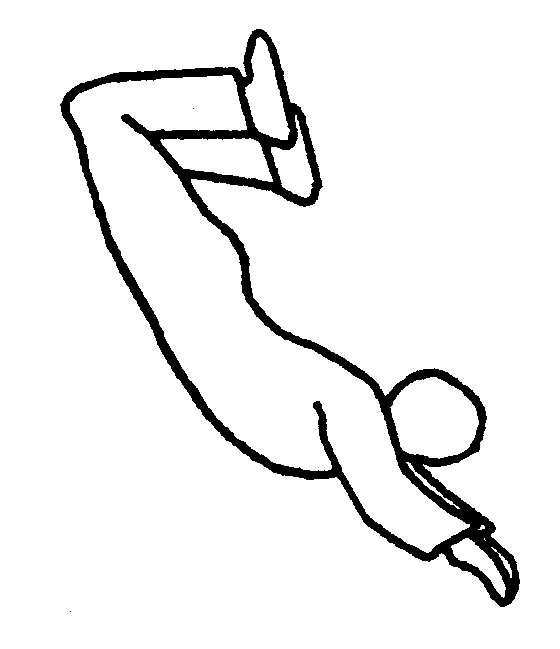
\includegraphics[width=0.7\textwidth]{UH-sukellus.png}\captionof{figure}{Sukellusuloshyppy}\end{Figure} 

\subsection{ Streevakone }
\label{uloshyppytyylit-streevakone}

\begin{enumerate}[label=\bfseries \arabic*)]
\item  Oikea jalka astimelle, varpaat peräsimen suuntaan. 
\item  Kädet oviaukon reunalle. 
\item  Kohottaudutaan (varoen repun osumista koneeseen) koneen ulkopuolelle. 
\item  Käännytään koneen peräsintä kohti. 
\item  Sukelletaan ilmavirran suuntaan taaksepäin, rinta ilmavirtaan. 
\item  Taivutus, pää taakse, jalat koukkuun taakse ja kädet eteen leveälle. 
\item  Sitä mukaan kun asento kääntyy vaakatasoon (tyypillisesti noin 5 sekunnin jälkeen) otetaan perusasento. 
\end{enumerate}
\subsection{ Muut koneet }
\label{uloshyppytyylit-muut-koneet}

\begin{enumerate}[label=\bfseries \arabic*)]
\item  Siirrytään oviaukolle (varoen repun osumista koneeseen) kyykkyyn tai seisaalleen. 
\item  Sukelletaan ilmavirran suuntaan taaksepäin, rinta ilmavirtaan. 
\item  Taivutus, pää taakse, jalat koukkuun taakse ja kädet eteen leveälle. 
\item  Sitä mukaan kun asento kääntyy vaakatasoon (tyypillisesti noin 5 sekunnin jälkeen) otetaan perusasento. 
\end{enumerate}
\subsection{ Ongelmat }
\label{uloshyppytyylit-ongelmat}

\begin{enumerate}[label=\bfseries \arabic*)]
\item  Ponnistus sivulle aiheuttaa kaatumisen kyljelleen. 
\item  Rintamasuunnan ollessa muutoin kuin ilmavirtaan, asento kaatuu. 
\item  Epäsymmetrinen raajojen asento aiheuttaa kääntymistä, voltin tai syöksyn. 
\end{enumerate}
\section{ Ryhmäuloshyppy }
\label{uloshyppytyylit-ryhmauloshyppy}


Uloshypyn toteutus riippuu hyppääjien määrästä ja hyppykoneesta, mutta onnistuakseen uloshypyn täytyy aina olla yhdenaikainen ja hyppääjien lähtöasennon ilmavirran mukainen. Yhdenaikaisuus saadaan uloshyppylaskennalla, jonka yksi hyppääjistä aloittaa (ready) ja johon muut tulevat mukaan (set, go). Oikea lähtöasento, eli vatsan kääntäminen kohti ilmavirtaa, mahdollistaa hyvän lentoasennon heti uloshypystä lähtien. Jos sekä lähtöasento että yhdenaikaisuus epäonnistuvat, ei uloshyppy onnistu. Uloshyppyä tulee harjoitella yhtä paljon kuin itse vapaapudotusta, koska rauhallinen onnistunut hyppy alkaa hyvästä uloshypystä, kun taas epäonnistunut uloshyppy tuhlaa paljon vapaapudotussekunteja. 


Streevalla tai pyörällä istuminen on ehdottomasti \textbf{kielletty}. 


\begin{Figure}\centering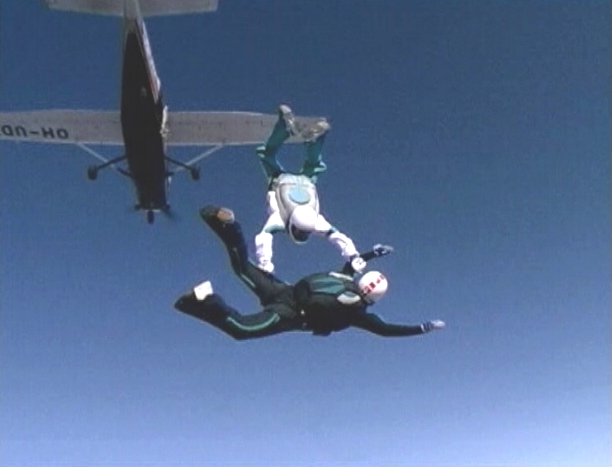
\includegraphics[width=0.95\textwidth]{UH-FS.jpeg}\captionof{figure}{FS-uloshyppy}\end{Figure} 

\section{ Muut uloshypyt }
\label{uloshyppytyylit-muut-uloshypyt}


Hyppääminen muista ilma-aluksista kuten helikoptereista, kuumailmapalloista jne. vaatii aina ennakkoharjoittelua. Perustapana on seisaalta pudottautuminen suoraan alaspäin ilmavirran suuntaan suoralla tai sukellus uloshypyllä. 

\section{ Harjoitus }
\label{uloshyppytyylit-harjoitus}

\begin{enumerate}[label=\bfseries \arabic*)]
\item  Katsotaan eri uloshyppyjä Oppilaan Opas-videolta kouluttajan kanssa. 
\item  Mietitään kouluttajan kanssa miten hyppääjä/hyppääjät hyödyntävät suhteellista ilmavirtaa kussakin uloshyppytyylissä. 
\item  Harjoitellaan omalla hyppykoneella/konemallilla kouluttajan mallisuoritusten mukaan eri uloshyppyjä. 
\item  Omatoiminen harjoittelu koneella/konemallilla ja näyte hyppymestarille suorasta ja sukellusuloshypystä. 
\end{enumerate}
